%% March 2018
%%%%%%%%%%%%%%%%%%%%%%%%%%%%%%%%%%%%%%%%%%%%%%%%%%%%%%%%%%%%%%%%%%%%%%%%%%%%
% AGUJournalTemplate.tex: this template file is for articles formatted with LaTeX
%
% This file includes commands and instructions
% given in the order necessary to produce a final output that will
% satisfy AGU requirements, including customized APA reference formatting.
%
% You may copy this file and give it your
% article name, and enter your text.
%
%%%%%%%%%%%%%%%%%%%%%%%%%%%%%%%%%%%%%%%%%%%%%%%%%%%%%%%%%%%%%%%%%%%%%%%%%%%%
% PLEASE DO NOT USE YOUR OWN MACROS
% DO NOT USE \newcommand, \renewcommand, or \def, etc.
%
% FOR FIGURES, DO NOT USE \psfrag or \subfigure.
% DO NOT USE \psfrag or \subfigure commands.
%%%%%%%%%%%%%%%%%%%%%%%%%%%%%%%%%%%%%%%%%%%%%%%%%%%%%%%%%%%%%%%%%%%%%%%%%%%%
%
% Step 1: Set the \documentclass
%
% There are two options for article format:
%
% PLEASE USE THE DRAFT OPTION TO SUBMIT YOUR PAPERS.
% The draft option produces double spaced output.
%

%% To submit your paper:
\documentclass[draft,linenumbers]{agujournal2018}
\usepackage{apacite}
\usepackage{url} %this package should fix any errors with URLs in refs.

%%%%%%%
% \usepackage{trackchanges}
% uncomment the line above to use the TrackChanges package to mark revisions if needed.
% The trackchanges package adds five new LaTeX commands:
%
%  \note[editor]{The note}
%  \annote[editor]{Text to annotate}{The note}
%  \add[editor]{Text to add}
%  \remove[editor]{Text to remove}
%  \change[editor]{Text to remove}{Text to add}
%
% complete documentation is here: http://trackchanges.sourceforge.net/
%%%%%%%

\draft

% Now, type in the journal name: \journalname{<Journal Name>}

% ie, \journalname{Journal of Geophysical Research}
%% Choose from this list of Journals:
%
% JGR-Atmospheres
% JGR-Biogeosciences
% JGR-Earth Surface
% JGR-Oceans
% JGR-Planets
% JGR-Solid Earth
% JGR-Space Physics
% Global Biochemical Cycles
% Geophysical Research Letters
% Paleoceanography
% Radio Science
% Reviews of Geophysics
% Tectonics
% Space Weather
% Water Resource Research
% Geochemistry, Geophysics, Geosystems
% Journal of Advances in Modeling Earth Systems (JAMES)
% Earth's Future
% Earth and Space Science
% Geohealth
%

\journalname{Water Resource Research}

\usepackage{textgreek}
\usepackage{natbib}
\begin{document}

%% ------------------------------------------------------------------------ %%
%  Title
%
% (A title should be specific, informative, and brief. Use
% abbreviations only if they are defined in the abstract. Titles that
% start with general keywords then specific terms are optimized in
% searches)
%
%% ------------------------------------------------------------------------ %%

% Example: \title{This is a test title}

\title{An Implementation of a Convolutional Neural Network for Fast Segmentation of 4D Microtomography Volumes from Core-flooding Experiments in Porous Rock}

%% ------------------------------------------------------------------------ %%
%
%  AUTHORS AND AFFILIATIONS
%
%% ------------------------------------------------------------------------ %%

% Authors are individuals who have significantly contributed to the
% research and preparation of the article. Group authors are allowed, if
% each author in the group is separately identified in an appendix.)

% List authors by first name or initial followed by last name and
% separated by commas. Use \affil{} to number affiliations, and
% \thanks{} for author notes.
% Additional author notes should be indicated with \thanks{} (for
% example, for current addresses).

% Example: \authors{A. B. Author\affil{1}\thanks{Current address, Antartica}, B. C. Author\affil{2,3}, and D. E.
% Author\affil{3,4}\thanks{Also funded by Monsanto.}}

\authors{Y.Yang, S.Seth, I.B.Butler, F.Fusseis....}


% \affiliation{1}{First Affiliation}
% \affiliation{2}{Second Affiliation}
% \affiliation{3}{Third Affiliation}
% \affiliation{4}{Fourth Affiliation}

\affiliation{1}{University of Edinburgh}
%(repeat as many times as is necessary)

%% Corresponding Author:
% Corresponding author mailing address and e-mail address:

% (include name and email addresses of the corresponding author.  More
% than one corresponding author is allowed in this LaTeX file and for
% publication; but only one corresponding author is allowed in our
% editorial system.)

% Example: \correspondingauthor{First and Last Name}{email@address.edu}

\correspondingauthor{Yili YANG}{yili.yang@ed.ac.uk}

%% Keypoints, final entry on title page.

% Example:
% \begin{keypoints}
% \item	List up to three key points (at least one is required)
% \item	Key Points summarize the main points and conclusions of the article
% \item	Each must be 100 characters or less with no special characters or punctuation
% \end{keypoints}

%  List up to three key points (at least one is required)
%  Key Points summarize the main points and conclusions of the article
%  Each must be 100 characters or less with no special characters or punctuation

\begin{keypoints}
\item Machine learning segmentation enables fast segmentation with compromised data quality and reduces processing time from few hours to few minutes
\item Machine learning segmentation has resistance to noise and ring artefacts
\item Machine learning segmentation is applicable to large time resolved data sets such as those from synchrotron time resolved microtomography

\end{keypoints}

%% ------------------------------------------------------------------------ %%
%
%  ABSTRACT
%
% A good abstract will begin with a short description of the problem
% being addressed, briefly describe the new data or analyses, then
% briefly states the main conclusion(s) and how they are supported and
% uncertainties.
%% ------------------------------------------------------------------------ %%

%% \begin{abstract} starts the second page

\begin{abstract}
Multiphase fluid flow in porous media is extensively studied for its applications in carbon capture and storage, hydrocarbon recovery, aquifer contamination, soil hydrology and subsurface energy resources. Fluid displacement in porous media can be investigated using highly time-resolved synchrotron x-ray microtomography. One consequence of extremely fast imaging can be compromised image quality, including noise and decreased contrast, which makes images hard to segment. We implemented a convolutional neural network (CNN) and trained it with 14k+ images from multiphase flow experiments generated by synchrotron \textmu CT. The trained neural network can segment synchrotron \textmu CT images of core-flooding experiments fast and accurately without any pre-processing of the raw image. Segmenting one \textmu CT volume of size 1003x496x496 takes about 10 minutes on a Nvidia Quadro K5200 GPU, while conventional methods (watershed) using CPU for the same data takes 2.5 hours (pre-processing and denoising time included for comparison). On the test data set, the AUC-ROC score of individual class reached above 0.99 and mean accuracy of the three segmentation class reached 0.99. The accuracy of the CNN segmentation is the same order as conventional methods but speed is significantly enhanced.
\end{abstract}


%% ------------------------------------------------------------------------ %%
%
%  TEXT
%
%% ------------------------------------------------------------------------ %%

%%% Suggested section heads:
% \section{Introduction}
%
% The main text should start with an introduction. Except for short
% manuscripts (such as comments and replies), the text should be divided
% into sections, each with its own heading.

% Headings should be sentence fragments and do not begin with a
% lowercase letter or number. Examples of good headings are:

% \section{Materials and Methods}
% Here is text on Materials and Methods.
%
% \subsection{A descriptive heading about methods}
% More about Methods.
%
% \section{Data} (Or section title might be a descriptive heading about data)
%
% \section{Results} (Or section title might be a descriptive heading about the
% results)
%
% \section{Conclusions}
\section{Introduction}
Experimental studies of fluid flow related processes in porous media, including multiphase flow and reactive flow, have increasingly made use of x-ray microtomography (\textmu CT) techniques to image fluid distributions and changes in porous media in-situ. These studies range from those which employ laboratory \textmu CT instruments (e.g. \citet{pak2015droplet,alratrout2018wettability}) to those which employ synchrotron \textmu CT to generate 4D time resolved data which reveal processes in action (e.g. \citet{berg2014multiphase,reynolds2017dynamic,berg2013real}). The high photon flux at synchrotron x-ray sources enables experimenters to acquire multiple \textmu CT volumes, each scan lasting few seconds or less, over minutes to hours of experimentation. With 4D data sets often approaching a few terabytes and comprising many 10s to 100s of discrete data volumes, the efficiency of image processing and segmentation can present a bottleneck to downstream data analysis. Furthermore, fast scans with brief exposure times and few projections, combined with progressive damage to scintillators resulting from high X-ray fluxes may lead to increased noise, image artifacts and low contrast, making image classification and segmentation difficult and time consuming.

In this contribution we trained a convolutional neural network (CNN) to efficiently segment synchrotron \textmu CT images obtained during core-flooding experiments. The images comprise three classes of objects: rock, oil and water. The trained CNN network is able to segment the three phases directly from reconstructed images accurately and rapidly without pre-processing steps such as application of noise filters. 

The CNN implementation that we present herein is developed specifically for fast, efficient, segmentation of large numbers of 3D volumes acquired through time resolved microtomographic imaging of two or more fluid phases within a porous medium. It can reduce processing times 15-fold compared to conventional segmentation methods. This approach of using machine learning to handle large volume segmentation can be applied as a 
generic method to more types of \textmu CT imaging data.

\subsection{Segmentation using convolutional neural network}
Unlike conventional segmentation methods that only take single, or simple combination of features into account, deep learning neural networks allows abstraction of multiple levels of features, such as curves, lines and even complex patterns of data, and use such features to make segmentation. Convolutional neural networks (CNNs, \citet{lecun2015deep}) are a class of deep neural network that have been proved effective in visual recognition tasks (e.g. \citet{krizhevsky2012imagenet}; \citet{long2015fully};\citet{girshick2014rich}). \citet{ronneberger2015u} also proved the reliability of CNN in segmenting low-contrast gray scale biomedical images, which are similar to our experimental multiphase flow data that are also gray scale images with low-contrast objects. For this reason, we have chosen to use the CNN architecture 'U-Net' introduced by \citet{ronneberger2015u}, to train a segmentation model and yielded accurate and precise segmentation.

The training of a CNN model is a form of supervised learning. The purpose of training is to use limited data to train a generalized model to classify all data of this type. During training, the model is trying to learn the knowledge of 'how to classify pixels into oil, water, and solid', input training data are the 'exercise', prediction is the machine's 'answer', and labelled data is the 'ground truth', loss function is the scoring criteria and loss value is the score of the 'exercise'. By iteratively doing a large amount of 'exercise', the machine can eventually learn to classify pixels correctly by optimising the loss value.

However, when the training data set is excessively iterated, the model becomes too specific to the training data set and unable to make generalized prediction to data beyond the training set, this problem is called over-fit. For this reason, an independent validation data set is separated for cross-validation to prevent over-fit.

Validation is a process similar to training, performed at the end of each (or every few) training epoch. The difference is that the learning process is prevented, only the outcome of previous learning is examined. Validation can be used to check over-fit and tune hyper-parameters that control model's overall learning behaviour. 

When training is completed, a held-out test set is revealed to the CNN model to test its performance on entirely unfamiliar data. This set is absolutely 'unseen' by the CNN model so the test score can provide an unbiased evaluation of the reliability of the model prediction on real-world data. Evaluation criteria of image segmentation often include intersection over union (IoU), accuracy, precision, recall and F1 score etc. The evaluation scores represent the reliability of segmentation produced by the trained CNN model.

\subsection{Ground-truthing}\label{gtintro}
Unlike conventional images that contain objects such as animals, cars or human are with relatively smooth and simple boundary, pore scale experimental images have highly irregular, multi-scale, even fractal boundaries which make manual annotation very difficult and imprecise. In our studied experimental \textmu CT data, the manual annotation has mainly three problems 1) the highly irregular and multi-scale boundaries 2) similar grey scale for different objects, i.e., brine and rock. 3) heavy noise and artefacts. For the above reasons, we acquired the ground truth of the input images using a weakly supervised algorithm and carefully assessed that the segmentation achieved is sufficiently accurate and reliable. We used Scikit-image implementation of 'Seeded random-walker' \citep{grady2006random} algorithm. The overall segmentation process is computationally expensive and not scale-able. Our goal is to reproduce this segmentation process by deep learning to achieve accurate, fast and scale-able result. Details of the ground-truthing method is described in \ref{gtmethod}.

\section{Materials and methods}
\subsection{Multiphase fluid flow experiments}
A benchmark carbonate rock, Indiana limestone, was used as porous medium in the experiments.The rock was cored and installed in an X-ray transparent cell designed by \citet{fusseis2014low}. For fluid injection we used mineral oil and Potassium Iodine solution as oil and aqueous phase respectively. Synchrotron X-ray Images were acquired using pink beam by one second acquisition time in every 20 seconds during fluid injections. We used the beam line 2-BM at the Advanced Photon Source in Argonne National Laboratory in Chicago, U.S.

\subsection{Ground truth segmentation}\label{gtmethod}
The \textmu CT projections (raw data acquired from \textmu CT scans) were reconstructed using filtered back projection method. The reconstructed images are referred to as 'raw \textmu CT images' that are essentially a sequence of horizontal cross-sectional image slices of the scanned object. The raw \textmu CT images are the input images for the CNN segmentation. Shown in Fig.\ref{prep} upper left, the raw \textmu CT image has three target phases (inside the cylindrical rock core) marked in red boxes as examples: the dark grey is oil, the light grey is brine, and also light grey but with higher relief on the boundary is rock. Due to the complex nature of the pore-scale \textmu CT images described in \ref{gtintro}, we acquired the ground truth images by a processing workflow described below:

With a high-resolution reference dry scan (before fluid injection) available, we threshold-ed the solid phase and used it as mask in wet scans to further separate the two fluid phases, the mask was registered and applied using Avizo9\texttrademark. Fig.\ref{prep} upper right shows the raw \textmu CT images after rock mask applied. The rock-brine-oil system now is more distinguishable, but the brine and oil are still very noisy.
 
We used non-local Means \citep{buades2005non} filter to denoise the rest of the two phases in the masked images (Fig.\ref{prep} lower left). We used ImageJ implementation of the filter and used sigma value 30 and default window size. The brine and oil are free-of-noise at this stage, but the side-effect comes that the object boundary is blurry. The denoising for data volume size $1004\times1646\times1646$ took 1 hour to finish.

We implemented the seeded random-walker algorithm \citep{grady2006random} to finalize the ground-truthing. Seeded random walker is a region growing method which good at inferring ambiguous boundaries. Implementation in Scikit-image was used and averagely took 119 minutes performing in 3D. Seed-generating threshold value used for the upper and lower boundaries of the middle phase was 143 and 129. Beta value used for seed diffusion difficulty was 200.

The random analytical error for ground truth are determined as two standard deviations (2\textsigma) of the sum of fluid volumes and the total pore volume measured based on image, which is 1.86\% based on the conservation of pore space. Besides small error on bulk volume, we also checked details of pore structures and fluid arrangement slice by slice with the raw \textmu CT image, and guaranteed that the difference between ground truth segmentation and genuine ground truth is insignificant.

Although rather accurate, the whole segmentation work flow is very time-consuming (3+ hours per volume) and used different software thus difficult to automate. The parameters are also hand-tuned which costed a great amount of time. This segmentation workflow is not scale-able not only because of the high time and computational cost, but also the same parameters are not applicable over two batch of scans. We acquired a total of 144 \textmu CT scans during the experiment, and used only 14 \textmu CT scans (containing 14k + images) to train the segmentation neural network, the investment of training time is significantly profitable in terms of saving future time for \textmu CT data segmentation.

\begin{figure}[h]
\centering
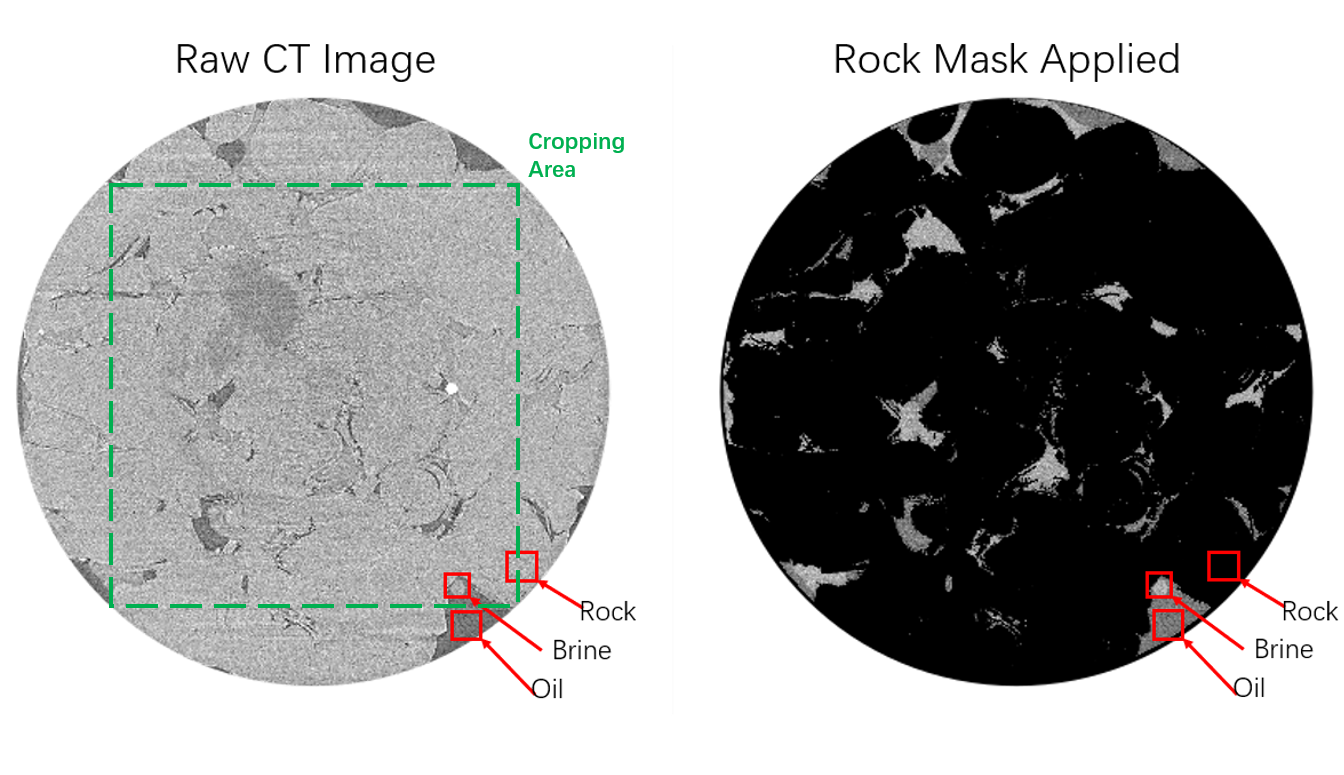
\includegraphics[width=33pc]{imgs/raw-masked2.png}
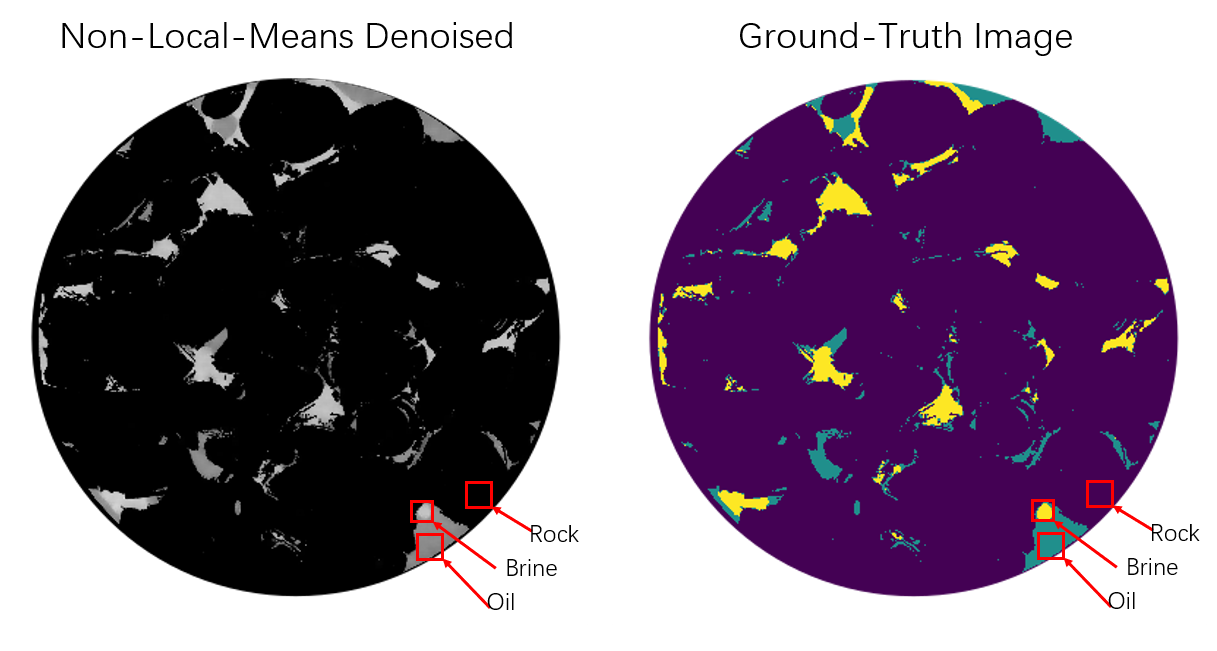
\includegraphics[width=33pc]{imgs/nlm-gt2.png}
\caption{The image segmentation work flow for ground-truthing. Upper left: raw \textmu CT image containing three object phases: oil, brine and rock. The fluid phases are hardly distinguishable because the rock has similar intensity with the brine. Green box shows the cropped area that used as network input. Upper left: the raw \textmu CT image with rock masked as black with the rock segmentation acquired from a dry reference scan, this makes further segmentation of two fluid phases possible. Lower left: masked image filtered by the non-local-means algorithm to reduce the noise. Lower right: ground truth segmentation produced by seeded random-walker algorithm.}
\label{prep}
\end{figure}

\subsection{Convolutional neural network segmentation}
\subsubsection{Data preparation}
Every original reconstruction image was paired with the corresponding ground truth image to make a pair of input-target image set for the network training. A total of 18 \textmu CT volumes were divided into 14 training sets, 2 test sets and 2 validation set. Each \textmu CT volume has 1003 reconstruction images. The cylindrical core images ($1646\times1646$) were sub-sampled ($736\times736$) and cropped to size 496x496 to adapt to the limited GPU memory. The cropped area is shown in green box in Fig.\ref{prep}.

\subsubsection{Training methods}
We used the CNN architecture U-net introduced by \citet{ronneberger2015u} and implemented by \citet{Jorispytorch} using the open-sourced deep learning platform Pytorch (\citet{paszke2017automatic}). 

The network consists a contracting path (Fig.\ref{unet} left box) and an expansive path (Fig.\ref{unet} right box). The contracting path, like conventional CNN, uses $3\times3$ convolution, followed by ReLU, then $2\times2$ max pooling for down-sampling. 

The expansive path up-samples the feature map with $2\times2$ up-convolution, each followed by $3\times3$ convolution with ReLU. A concatenation of feature map of the corresponding contracting path is applied to the up-convoluted feature map (Fig.\ref{unet} grey arrow copy and crop). The concatenation of cropped feature map from contracting path is necessary for compensating the lost border pixels during convolution. U-net does not have any fully connected layer, the final $1\times1$ convolution maps the total 64-component feature vectors to the desired number of classes. 

\begin{figure}[h]
\centering
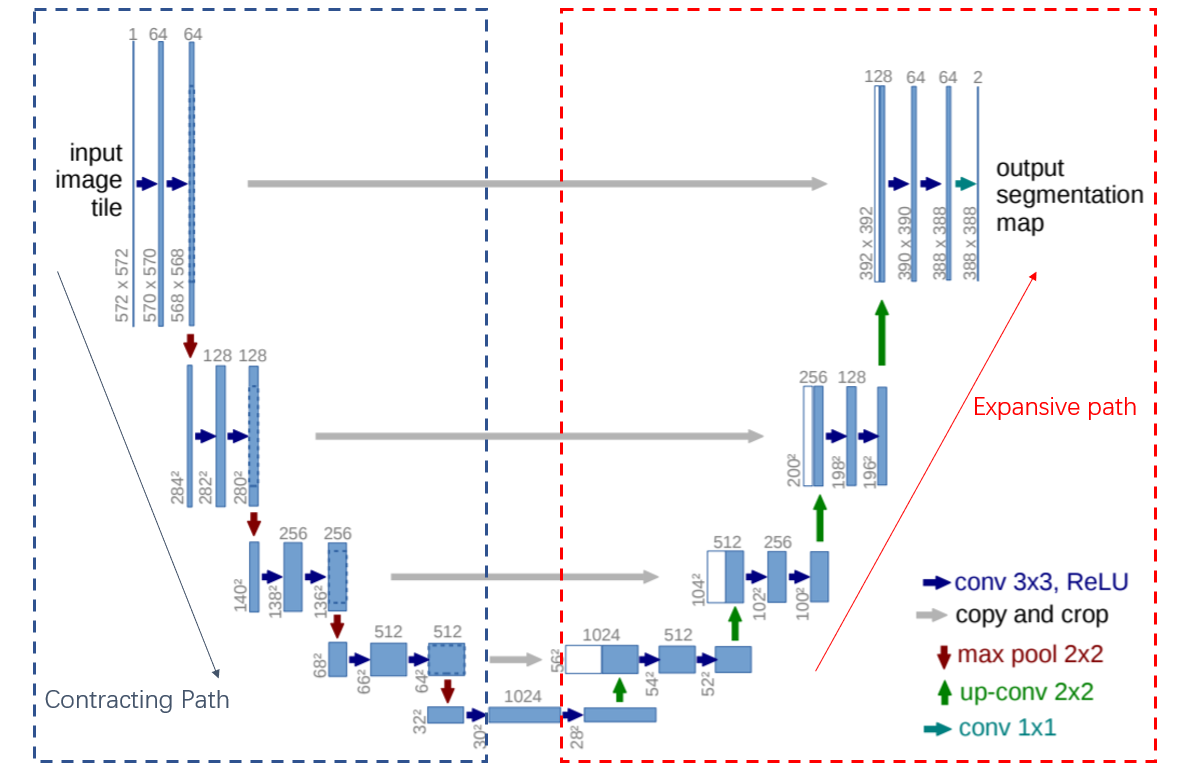
\includegraphics[width=33pc]{imgs/unet.png}
\caption{Modified from \citet{ronneberger2015u}, this figure shows the architecture of the U-net. It consists of a contracting path that extract different levels of features, and an expansive path that up-convolutes the image to produce the final segmentation. The two paths formed a U-shaped network}
\label{unet}
\end{figure}

In training (Fig.\ref{workfl} Training), the model takes a training image as input and produce a prediction of probability of each pixel belonging to a category. Then the prediction is compared with the ground truth image, and yield a loss value (Training loss, Fig.\ref{workfl} Training) which quantifies the difference between prediction and ground truth. The model iteratively updates the internal adjustable parameters (i.e. neuron weights) as training proceeds, to minimize the loss therefore improve the prediction step-wisely. A training epoch is a full traverse of all training data, we trained the CNN model for 34 epochs, with an NVidia\texttrademark Quadro K5200 GPU (8GB) to train the network. 

\begin{figure}[h]
\centering
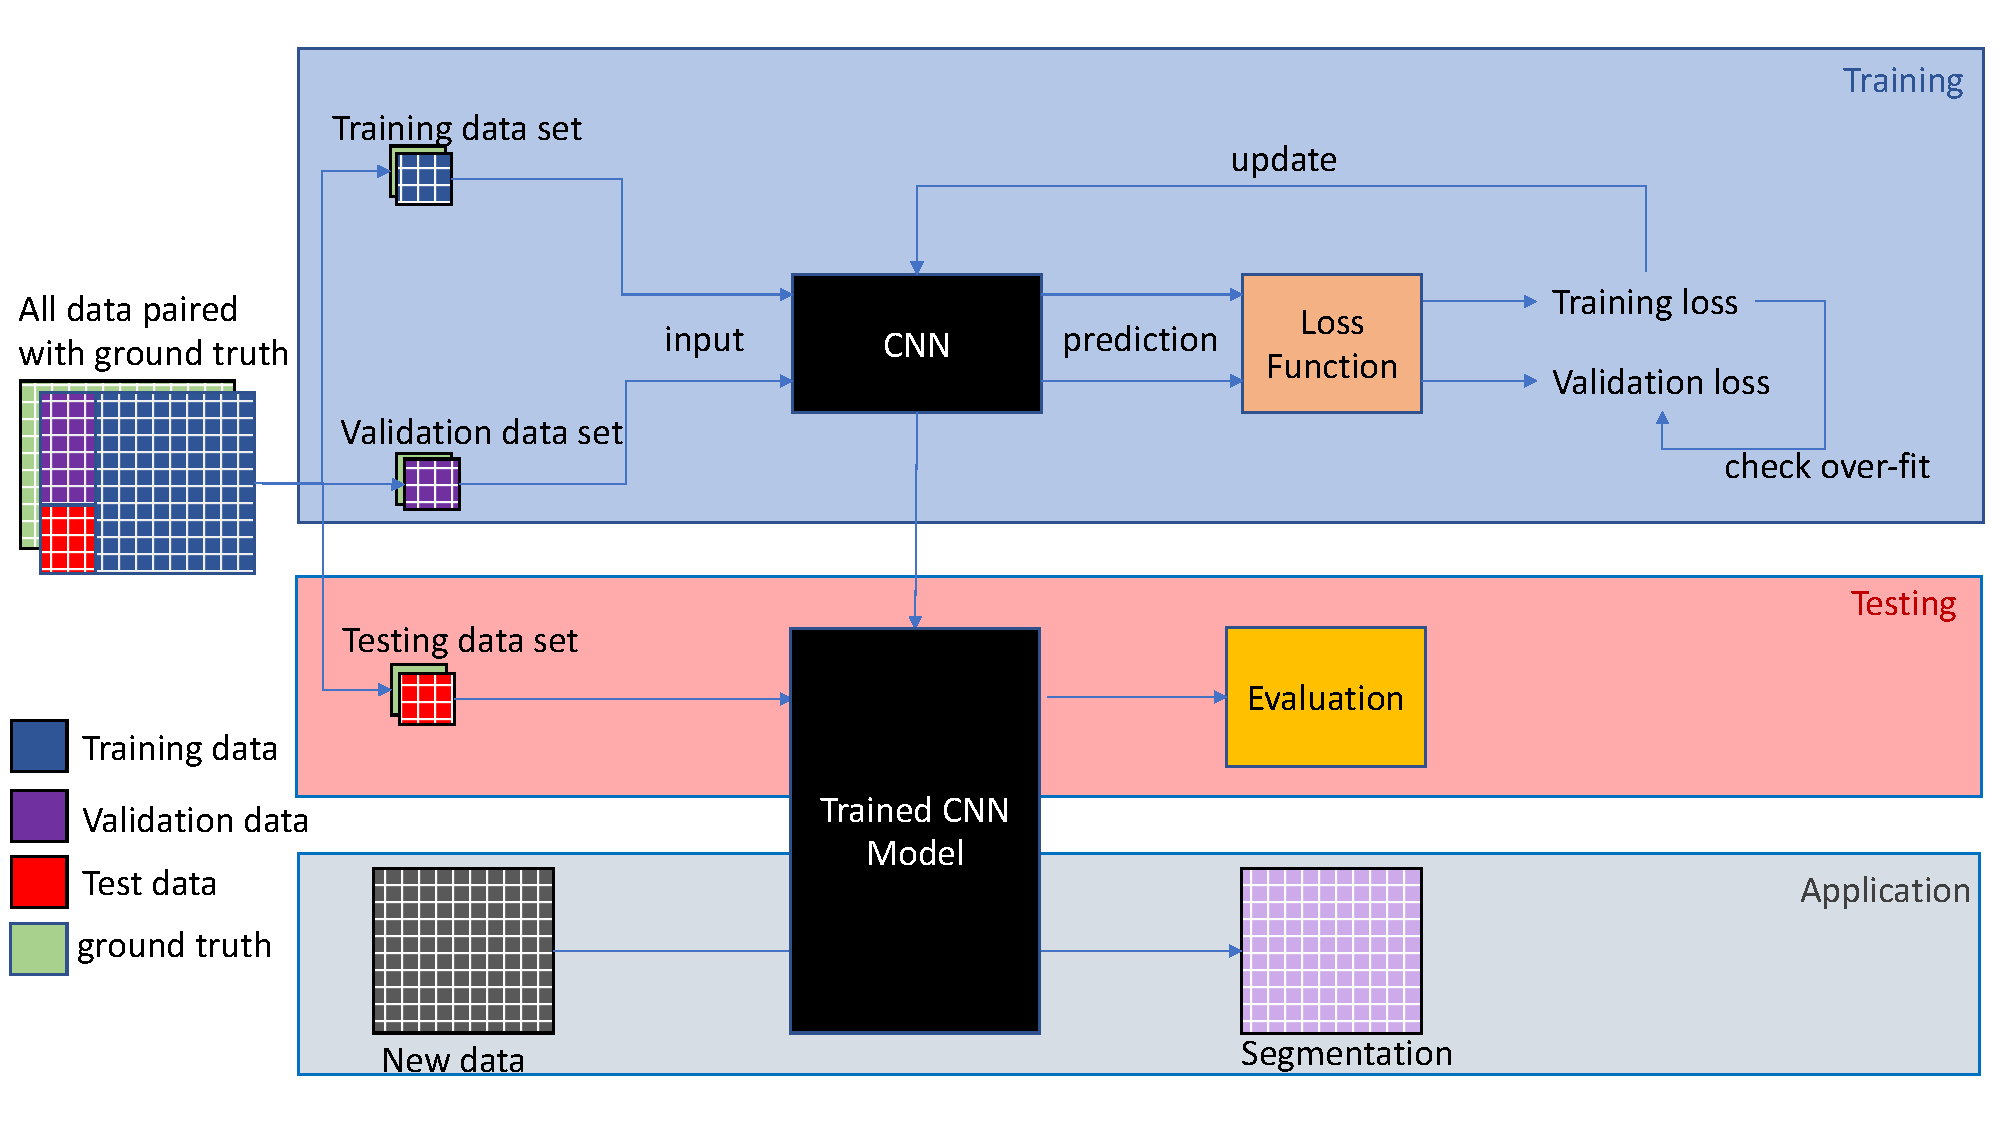
\includegraphics[width=33pc]{imgs/workfl.pdf}
\caption{CNN training, testing and application work flow. The training process uses training data set and validation data set to adjust the best fit of a CNN model that representing the relation between input images and ground-truth images. The testing process verify the model with a held-out data set. The application process uses the trained CNN model to segment new \textmu CT data.}
\label{workfl}
\end{figure}

Cross-entropy loss was used as the loss function during training. The loss function calculates the distance between the two probability distributions - the output prediction and the corresponding ground-truth. Cross-entropy decrease when the output and ground-truth have higher resemblance. The loss value was reduced step-wise during training and finally converged at the end of training. 

We used the Pytorch built-in cross-entropy loss function that is essentially a combination of Log-softmax function and Negative-log-likelihood loss function (NLL loss, also known as the multi-class cross-entropy \citep{bishop2006pattern}).

First the log-probability distribution of the network output is calculated using e.q.(\ref{lgsoftmax}):
\begin{linenomath*}
\begin{equation}\label{lgsoftmax}
    \centering
    \text{LogSoftmax}(x_{i}) = \log\left(\frac{\exp(x_i) }{ \sum_j \exp(x_j)} \right)
\end{equation}
\end{linenomath*}
where $x_i$ is the network output of the i-th class of all $j$ classes of image $x$. The result of e.q.(\ref{lgsoftmax}) is then passed into a NLL loss function e.q.(\ref{lossequation}) that calculates the mean NLL loss per-pixel. The loss, which is essentially the same expression as cross-entropy loss, can be written as:
\begin{linenomath*}
\begin{equation}\label{lossequation}
    \centering
    \text{Loss}(input, target) 
    = -input[target] + \log\left(\sum_j\exp(input_j)\right)
\end{equation}
\end{linenomath*}
where input and target are the model prediction and the ground truth. The target is one-hot coded.

The hyper-parameters are pre-defined parameters that control machine's overall learning behaviours during training. Multiple learning rates were tested and we found the value of $5\times10^{-5}$ is optimal for loss convergence. We used mini batch of 2 during training to train multiple slice in single iteration. L2 regularization $1\times10^{-5}$ was applied to alleviate over-fitting. The sequence of the input data was shuffled at the start of each epoch so that the neuron weights updated in each iteration were different, this helps with model's generalization. The optimizer used was Pytorch built-in Adam algorithm (\citet{kingma2014adam}) to accelerate training. 

\subsubsection{Validation}
At the end of each training epoch, the validation data set was input into the CNN. Similarly, the CNN yielded a prediction and then a loss value (Validation loss, Fig.\ref{workfl} Training). The validation loss was not back propagated to the CNN model, so it never learn from the validation set, this is to keep the validation set independent and unbiased. Because the learning is prohibited, it is impossible to over-fit the validation data set, so it can represent the lowest possible loss without over-fit.

The validation loss value is plotted throughout training and compared with the training loss value. The model is best-trained at the epoch when the validation loss starts to increase, or the validation accuracy stops to decrease, after the turning point the model becomes over-fit. 
 
We Rand accuracy \citep{rand1971objective} and area-under-curve of the receiver operating characteristic (AUC-ROC, \citet{bradley1997use}) as the metric of segmentation performance. Rand accuracy is the ratio of correctly classified pixels and total pixels. First we take probability above 95\% in prediction as true, then calculate the true positive (TP), false positive (FP), true negative (TN) and false negative (FN) w.r.t. the ground truth. The accuracy was calculated using eq.1:
\begin{linenomath*}
\begin{equation}
    accuracy=\frac{TP+TN}{TP+TN+FP+FN}
\end{equation}
\end{linenomath*}
The AUC-ROC is a common metric for assessing classification model's performance. ROC is a curve plotted in a coordinate system with true positive rate (Y-axis) against false positive rate (X-axis), at various threshold settings. ROC curve essentially represents the trade-off between sensitivity and specificity of a classification model. AUC as its name suggests, is the area under the ROC curve which measures the model's separability of different classes. AUC value is ranged between 0 and 1. When AUC value equals 1, it represents a perfect classification model that classify all true elements as true and all false elements as false. When AUC value equals 0, it represents a reversing model that classify all true elements as false and vice versa. When AUC value equals 0.5, it represents the worst case that all classifications are random due to completely overlapped probability distribution of trues and falses.

\subsubsection{Testing}
After training, it's necessary to test the performance of the CNN model on 'unseen' data to check its generalization and visually assess the segmentation quality on real-world data. The separated test data sets were first-time input into the trained neural network model (Fig.\ref{workfl} Testing). 

\section{Results}
\subsection{Training result}
Fig.\ref{crossval} shows the training process by plotting the validation accuracy and loss history. The upper image shows that as training proceeds, validation accuracy kept increasing and finally stabilized for all three phases. The lower image shows the validation loss plotted with the training loss. The training loss plunged at the outset of training and went less steep as the training proceeds. The validation error started at a relatively low position, but still decreased smoothly and slowly. The validation loss curve does not appear as the U-shaped paradigm, this is because the loss increment was subtle that made the curvature of the U-shape extremely large. Therefore the criterion we used for early-stopping is validation loss increasing for consecutively five epochs. The complete training set was trained for 34 epochs and the best fit was identified at the 29th epoch. The total training time was 205.4 hours. 

\begin{figure}[h]
 \centering
 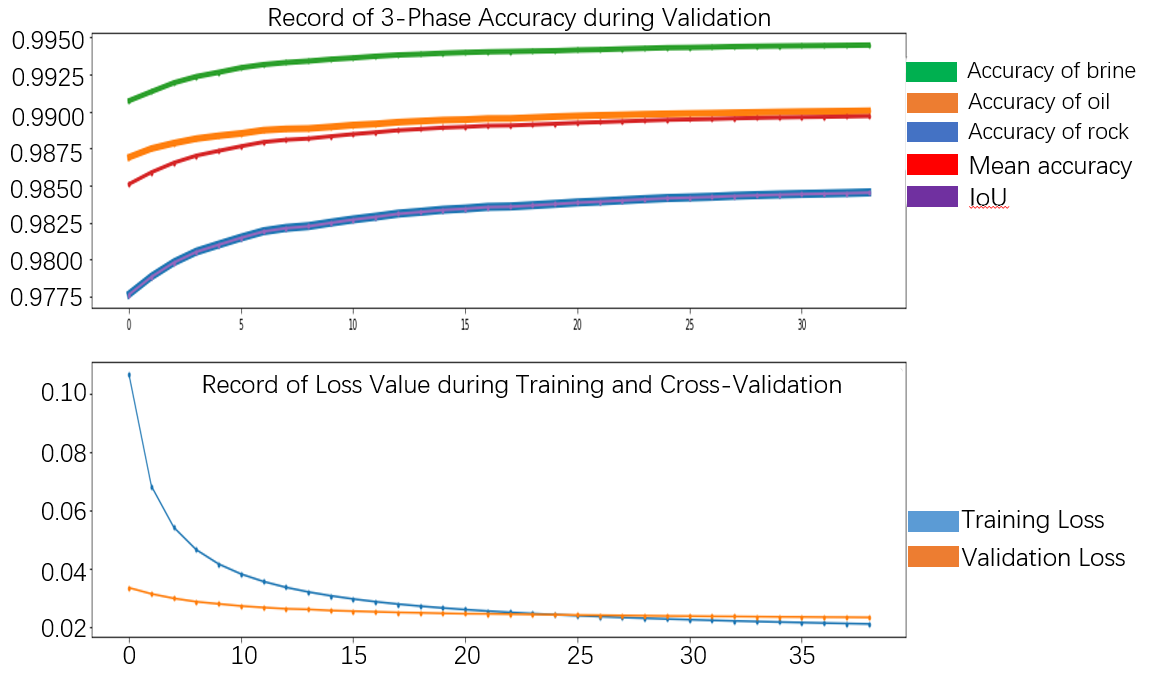
\includegraphics[width=33pc]{imgs/trainingresult_v1.png}
 \caption{Upper Image shows 3-phase individual accuracy improvement during validation. Lower image shows training loss and validation loss comparison during training. This illustrates the training and validation process of a CNN model, and the identification of the best-fit model.}
 \label{crossval}
 \end{figure}
 
 The model segmentation by the syn-training and trained model are shown in fig.\ref{1129}. The first row shows the raw testing image, the segmentation of the 11th epoch during training, and the ground truth. The second row shows the segmentation of the same image using the trained model, and the same ground truth. This implies the improvement of the model during training: at the 11th epoch the segmentation result is sub-standard, it only captures the skeleton of the pore space but the boundary decision is poor. On the 29th epoch the segmentation result is very similar to its ground truth. A full test of the final CNN model was performed using the 29th epoch model.
 
 \begin{figure}[h]
 \centering
 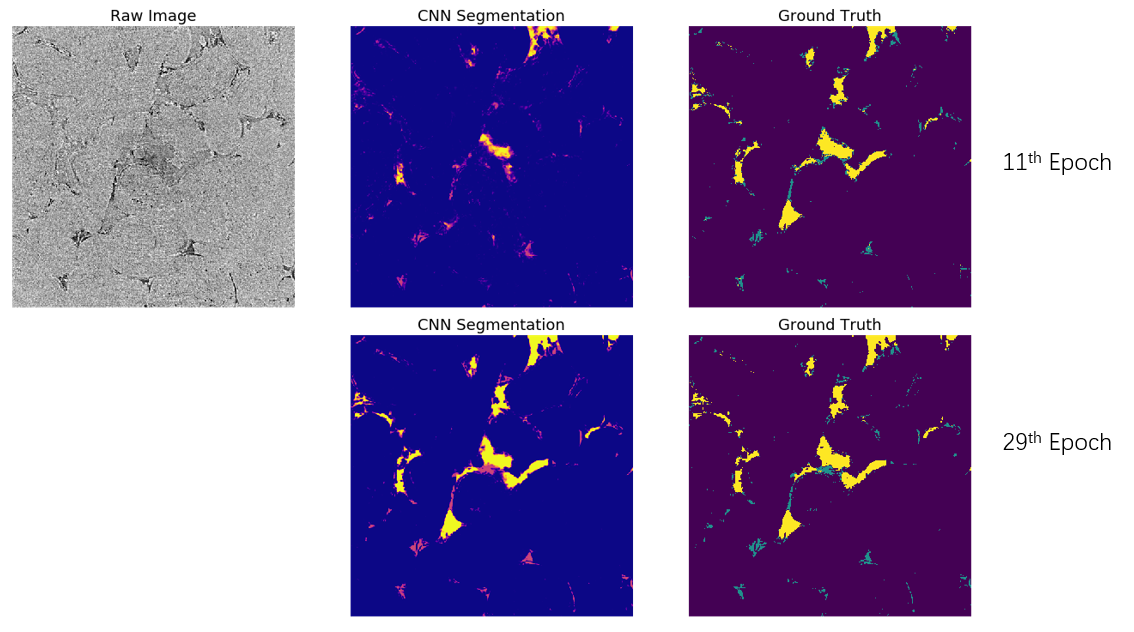
\includegraphics[width=33pc]{imgs/11-29.png}
 \caption{Segmentation result of the syn-training model at the 11th epoch, and the trained model at the 29th epoch. The CNN segmentation uses different color schemes than the ground truth for comparison. CNN segmentation uses blue-magenta-yellow for rock, oil and brine while the ground truth uses purple-darkcyan-yellow for rock oil and brine. The segmentation was on the same image from the testing data set. This illustrates the improvement of segmentation quality during training.}
 \label{1129}
 \end{figure}
 
\subsection{Testing Result of the trained network}
The model network trained for 29 epochs was identified as the best segmentation model and tested on the full testing data set. The performance measured on the test set shows high accuracy of all categories. The test result shows the accuracy of rock, brine, oil and mean are 98.51\%, 99.34\%, 99.16\% and 99.01\% respectively. Classification percentages are shown in the table \ref{clsfytable} below. 

\begin{landscape}\label{clsfytable}
\begin{table}[]
\centering
\begin{tabular}{|c|c|c|c|}
\hline
\multicolumn{1}{|r|}{Classification\%} & oil & brine & rock \\ \hline
oil & 93.627\% & 0.230\% & 6.142\% \\ \hline
brine & 0.358\% & 96.327\% & 3.316\% \\ \hline
rock & 0.392\% & 0.109\% & 99.498\% \\ \hline
\end{tabular}
\end{table}
\end{landscape}

Mean AUC-ROC score of individual segmentation phases are measured during testing. The AUC-ROC score for brine, rock and oil are 0.999, 0.999 and 0.998 respectively. It shows very high separability of the model.

The probability map (Fig.\ref{prob}) visualised the probability distribution of all three phases. It is generated by the softmax function that transforms the model output into a probability distribution of 0-1 distribution, and the probability of three phases of the same pixel add up to 1.  The colour map indicates the likeli-hood of a pixel belonging to one particular phase. The red end is extremely likely, the blue end is extremely unlikely, and white is ambiguous likeli-hood. The three phases are confidently determined because the ambiguous likely-hood pixels are of minor amounts, which mainly locate at the interface of two materials. It also illustrates a very robust performance of the model in segmentation. 

\begin{figure}[h]
 \centering
 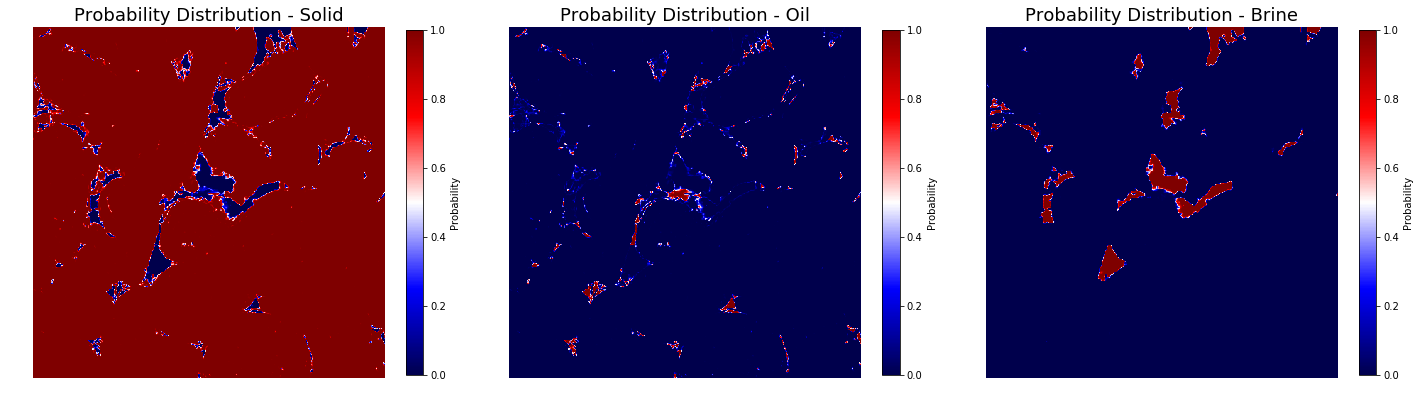
\includegraphics[width=33pc]{imgs/17_test_probmap.png}
 \caption{Probability distribution of phase segmentation. The coloured scale bar shows probability between 0-1, indicating the probability of a pixel that belongs to a specific segmentation category. This illustrates a determined segmentation with many certainties (probability close to 0 and 1) and very few uncertainties (probability around 0.5).}
 \label{prob}
 \end{figure}
 
The CNN model is completely trained and evaluated for very high segmentation performance. This model can be used to generate segmentation for new multiphase flow experimental data rapidly (Fig.\ref{workfl}. Application).

\begin{figure}[h]
 \centering
 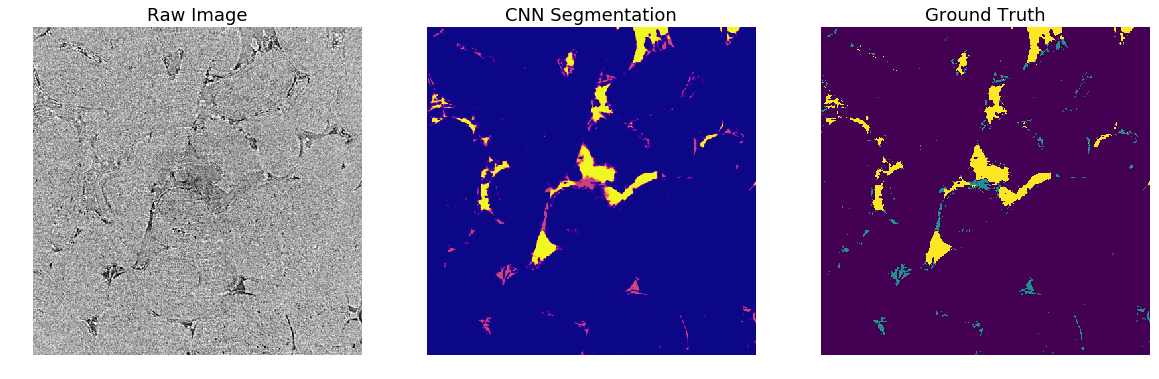
\includegraphics[width=33pc]{imgs/17_test_result.png}
 \caption{Comparison of input raw image, CNN segmentation result and ground truth. The raw image (left figure) is very noisy and can be segmented using a very complex and time-consuming work flow showing in Fig.1, to produce the ground truth image (right figure). The CNN model can segment the raw image directly into segmentation (middle figure) with significantly shorter time (few hours reduced to few minutes).}
 \label{result}
 \end{figure}

Taking probability above 95\% as foreground for each phase, the segmentation result is shown in Fig.\ref{result}. The visualization of CNN segmentation shows high similarity with ground truth. Minor differences existed but are hardly recognized visually. The result proves that the trained network is reliable in segmenting highly noised, low contrast \textmu CT reconstructed images.

External standards of the conservation of pore space (i.e. pore space is fixed over all time stamps) is also used to examine the test result. The experimental procedures ensure the pore space is filled with two fluids of either oil or brine, the proportion of the fluids can change through the experiments but the volume of oil and brine should always sum up to the pore space volume. Fig.\ref{accumulative} shows the accumulative phase pixels from the CNN segmentation and the ground truth. The sum of brine and oil pixels from CNN segmentation is 6,653,234 voxels. The ground truth sum, which equals to the pore space, is 6,975,417 voxels. The difference is 4.6\% which can be reckon as the segmentation error. The volume difference of CNN segmentation with ground truth for brine, oil and rock phase are +4.2\%, +5.3\% and less than -0.1\% respectively. 

To exclude data leakage that may occur when using highly similar training and testing data, we also tested the trained model on another \textmu CT data which from another experiment using the same rock and fluids. This \textmu CT volume is much later in the experimental time sequence, and has worse image quality compare with the training data set, due to technical limitation during long time imaging. The extra test results are: accuracy of rock=0.93\%,
accuracy of oil=0.95\%, accuracy of brine=0.99\%, mean accuracy=0.95\%. The performance remains a high level with only small decrease, which mainly due to worse imaging quality.

\section{Discussion}
\subsection{Extended Test}
To further examine the performance of the trained segmentation model on real data, the model was further tested on another data set of 20 scans which belongs to the same experimental set as the training data set but has later timestamps. The extended test data set was reconstructed using a different reconstruction tool Tomopy \citep{gursoy2014tomopy} and the image appearance was slightly different due to the different choice of reconstruction parameters. Therefore, the model was slightly biased with regard to the training data set. To balance the bias, the model was briefly trained for five epochs using only the first data of the 20. And tested with the rest of 19 data. The test result is shown in Fig.\ref{extendedtest}. The saturation of oil was measured from the segmentation produced by the CNN model and the ground truth which produced by the Random-walker algorithm. Kolmogorov–Smirnov test (K-S test, for non-normal distributions) was performed with the two saturation curves to examine if the two results are identical. The K-S test statistic result was 0.26 and the P-value was 0.54, both highly agrees with the null-hypothesis that the two results are identical. To conclude, the CNN segmentation model is able to produce reliable segmentation in practice, and has the ability to adapt to variations in the data set with minimum amount of re-train.

\begin{figure}[h]
 \centering
 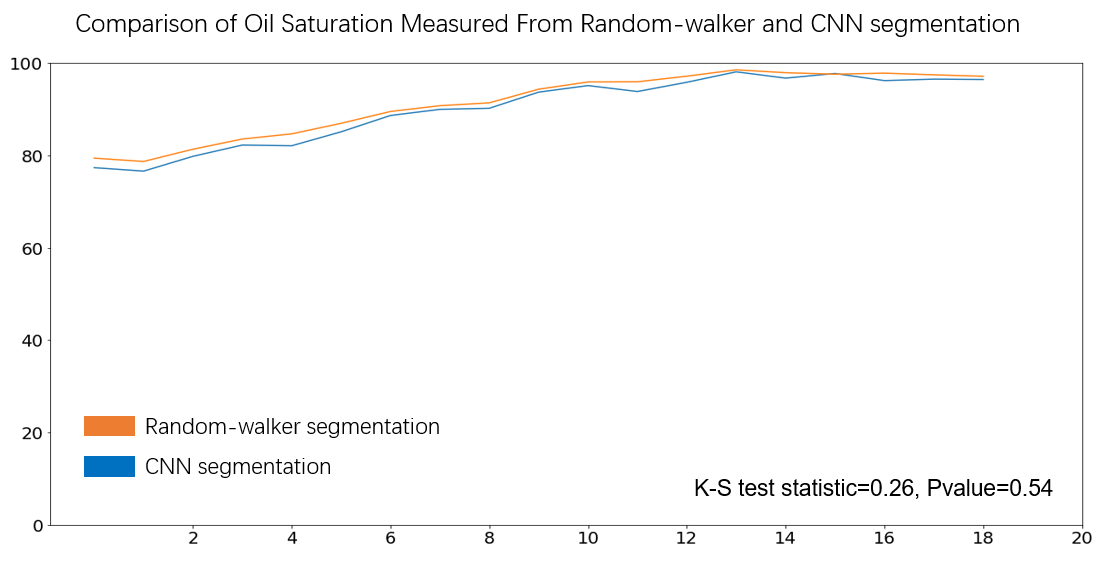
\includegraphics[width=33pc]{imgs/extendedtestresult.png}
 \caption{Oil saturation of consecutive 19 scan timestamps was measured from both CNN segmentation and Random-walker segmentation, and plotted as blue and orange curves respectively. The measurements of saturation from the segmentation using two methods are highly similar.}
 \label{extendedtest}
 \end{figure}


\subsection{Segmentation robustness test}
To test the robustness of the trained CNN model, we added three kinds of artificial image degradation to the a test image to test the model resistance to image quality degradation. The chosen test image is visually separable and does not suffer from severe \textmu CT imaging artefacts. The first image degradation series is blurring by convolving the image with a Gaussian function, it is essentially a smoothing or blurring process (Fig.\ref{noisetest} first row). The second type of image degradation is by adding Gaussian noise which is artificial noise with a probability distribution function of Gaussian distribution (Fig.\ref{noisetest} second row). The third type of image degradation is artificial ring artefact. Ring artefact is a common \textmu CT artefact that usually due to mis-calibration or failure of the detector element. Artificial ring artefact was generated by adding concentric circles with different radii and intensities at a fixed coordinate on the image. The index of ring artefact severeness is the number of iterations of generating circles (Fig.\ref{noisetest} third row).

\begin{figure}[h]
 \centering
 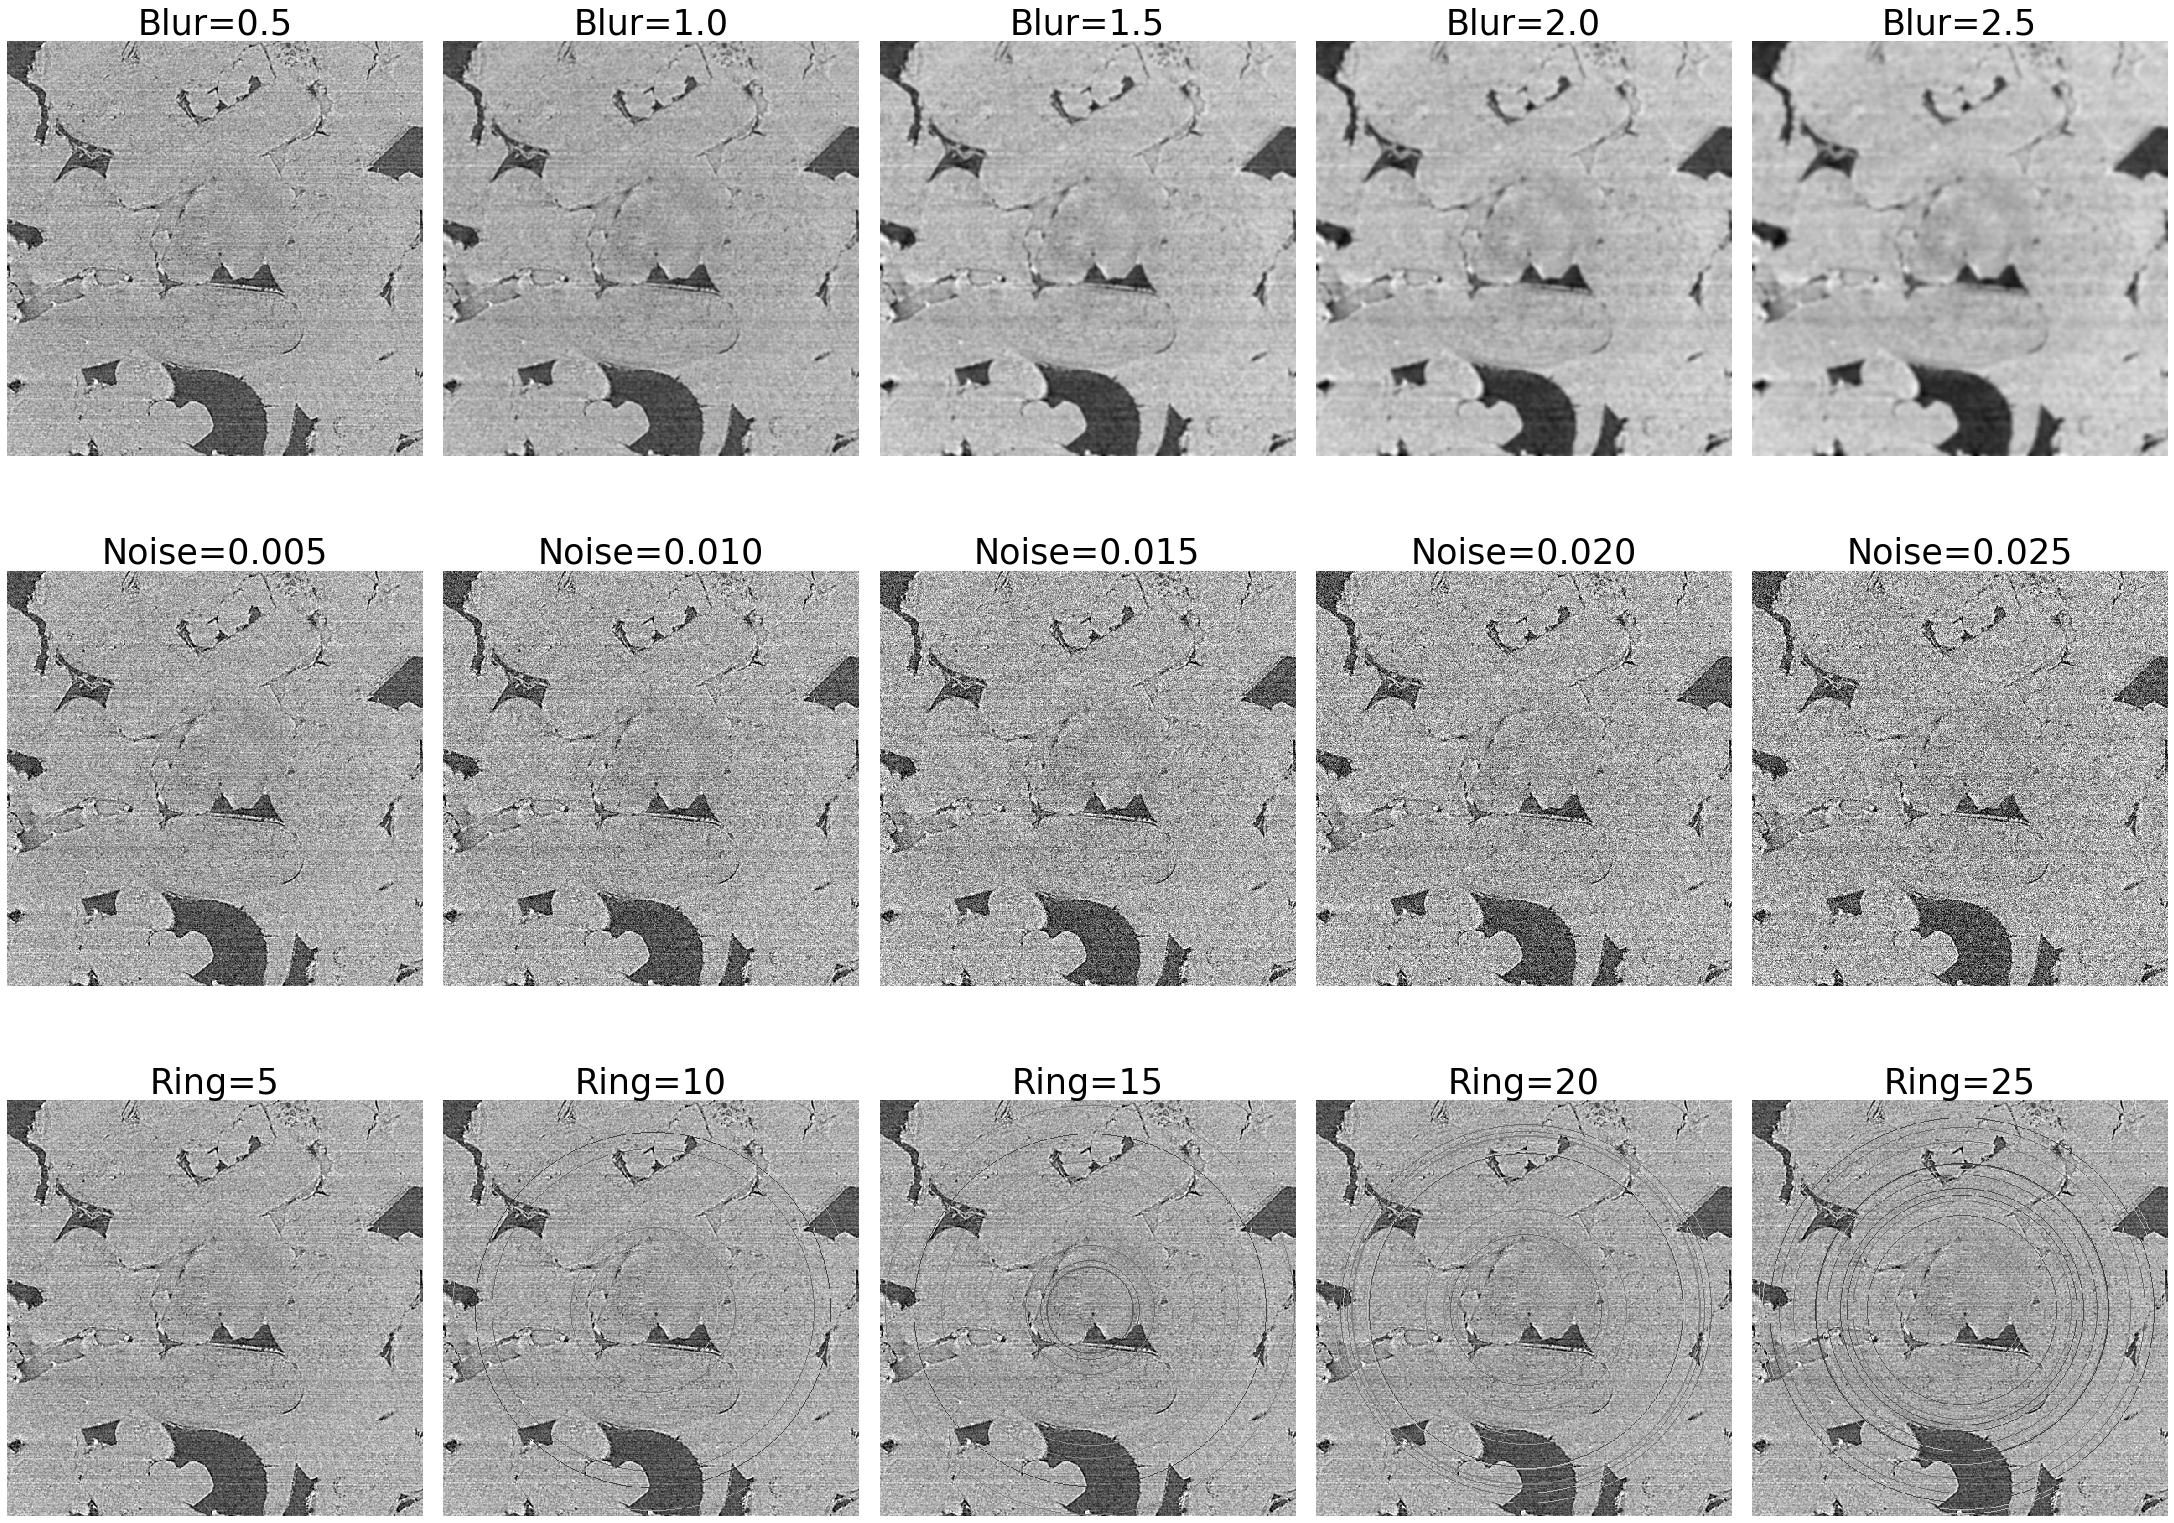
\includegraphics[width=33pc]{imgs/01dec_noisetest3}
 \caption{Image degradation series for testing the model resistance to image quality degradation: The first row is Gaussian blurring with sigma increment of 0.5, sigma is the standard deviation of the Gaussian distribution. The second row is Gaussian noising with sigma increment of 0.005. The third row is artificial ring artefact with number of rings increment of 5.}
 \label{noisetest}
 \end{figure}
 
 The image degradation series (Fig.\ref{noisetest}) was tested by the trained CNN model, and the segmentation results is shown below in Fig.\ref{misclassification}, with mis-classification marked in red circle. And the corresponding accuracy and AUC-ROC curve was plotted in Fig.\ref{robustness}.
 
 The result shows that, for the blurring series, the segmentation started to have major mis-classification since the second blurring step (blur=1.0). The model mis-classified oil as brine, and brine as rock, and oil as rock. It is surprising that even the most visually distinguishable features were mis-classified after adding some degree of blurring. The corresponding accuracy and AUC-ROC measurements in Fig.\ref{robustness} (upper) shows that the accuracy started to decrease after the second step of blurring, and then stabilized in further steps.
 
 For the noised images, all series are suffered from major mis-classifications regardless of the amount of noise added. All brine, oil and rock were massively mis-classified. This is also surprising, for the reason that the training data set has included many heavily noised images with no less noise than this test series. It means that Gaussian noise is not the type of noise that appeared on the training data set so the model still performs sub-standard on Gaussian noise. The corresponding accuracy measurement in Fig.\ref{robustness} (middle) shows the accuracy and AUC-ROC plunged since the first noising step and shows no sign of stabilising within the range of noise tested.
 
 The third type of image degradation is artificial ring artefacts. The CNN segmentation performed surprisingly well for this series. Only the last segmentation shows some minor mis-classification. The accuracy and AUC-ROC (Fig.\ref{robustness} (lower)) also agrees that the segmentation quality is highly stable and only decreased by a minor amount even with the highest ring artefact tested. It is also surprising because the training images do not have any significant ring artefacts. The positive result could be due to the fact that artificial rings actually affected much less pixels than the former two types.
 
 This test provides an insight on the CNN segmentation model sensitivity. The result implies that the model is highly sensitive to Gaussian type noise, and relatively lower sensitive to Gaussian type blurring. The model is highly insensitive to artificial ring artefacts. The result is surprising for that ring artefact seems the most severe and unsystematic degradation, from a human perspective. The blurring and noising however, have only limited impairment for human eye recognition. This indicates a very different way of recognising digital images by the state-of-art deep neural network model. This is indirectly supported by series of studies on computer vision of deep neural networks (i.e. \citet{nguyen2015deep, goodfellow2014explaining,su2019one}. The researches have found that the deep neural networks can be easily 'fooled' with some minor, but carefully crafted perturbations on the input image. \citet{goodfellow2014explaining} reported for example a panda image, when added with carefully constructed noise, is recognised as 'gibbon' with 99.3\% confidence, although the image still appears the panda to human eyes. \citet{su2019one} reported that with even one pixel altered by a particular way, the machine can make entirely wrong prediction in image classification. The other way around, \citet{nguyen2015deep} reported that a carefully crafted digital image pattern which makes zero sense to human, is recognised as a familiar object by deep neural network. In this study, the segmentation mis-classification due to Gaussian noising and blurring is not that extreme compared to the studies above, but the model network was still heavily influenced by these systematic, global modifications although the image appearance to human is far less. In contrast, the more local but unsystematic modification of the ring artefact, deals very little harm to the model prediction than it appear.
 
\begin{figure}[h]
 \centering
 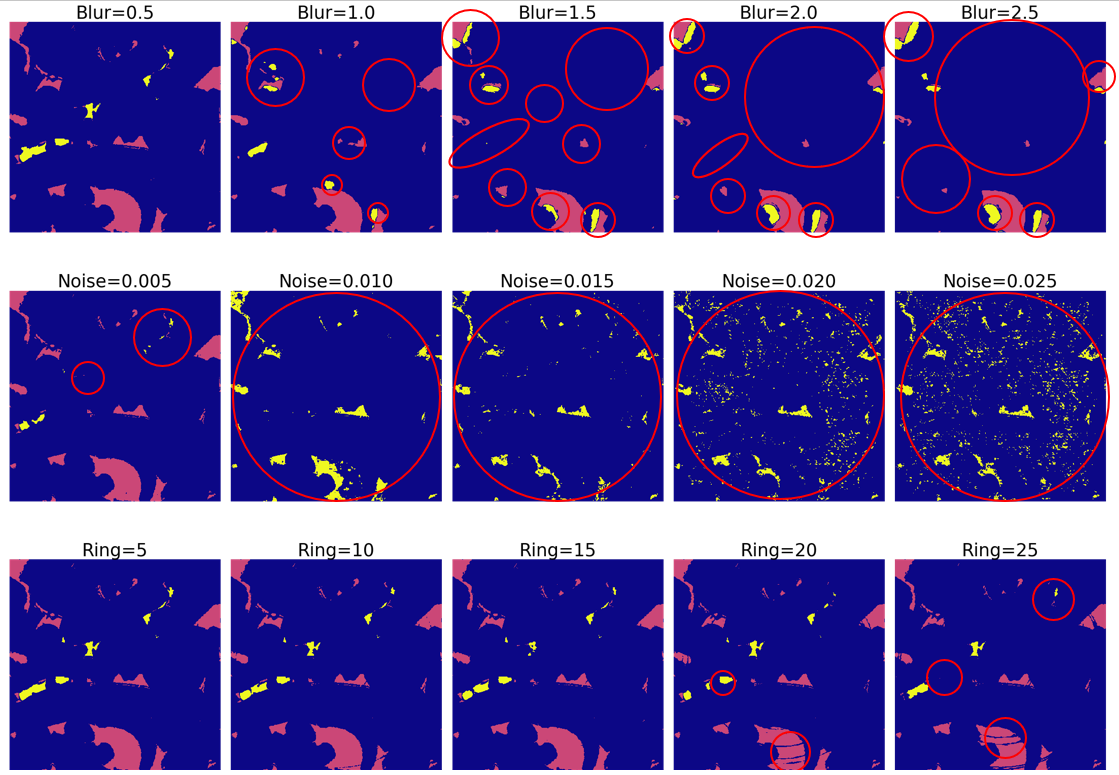
\includegraphics[width=33pc]{imgs/noisetest2.png}
 \caption{This figure shows the CNN segmentation of the corresponding degraded images of Fig.\ref{noisetest}. Major mis-classifications are identified in red circles. The result illustrates that the CNN model have different sensitivity to different types of image degradation. For the tested three types, Gaussian noise is highly sensitive, Gaussian blur is weakly resisted and artificial ring artefact is strongly resisted.}
 \label{misclassification}
 \end{figure}
 
\begin{figure}[h]
 \centering
 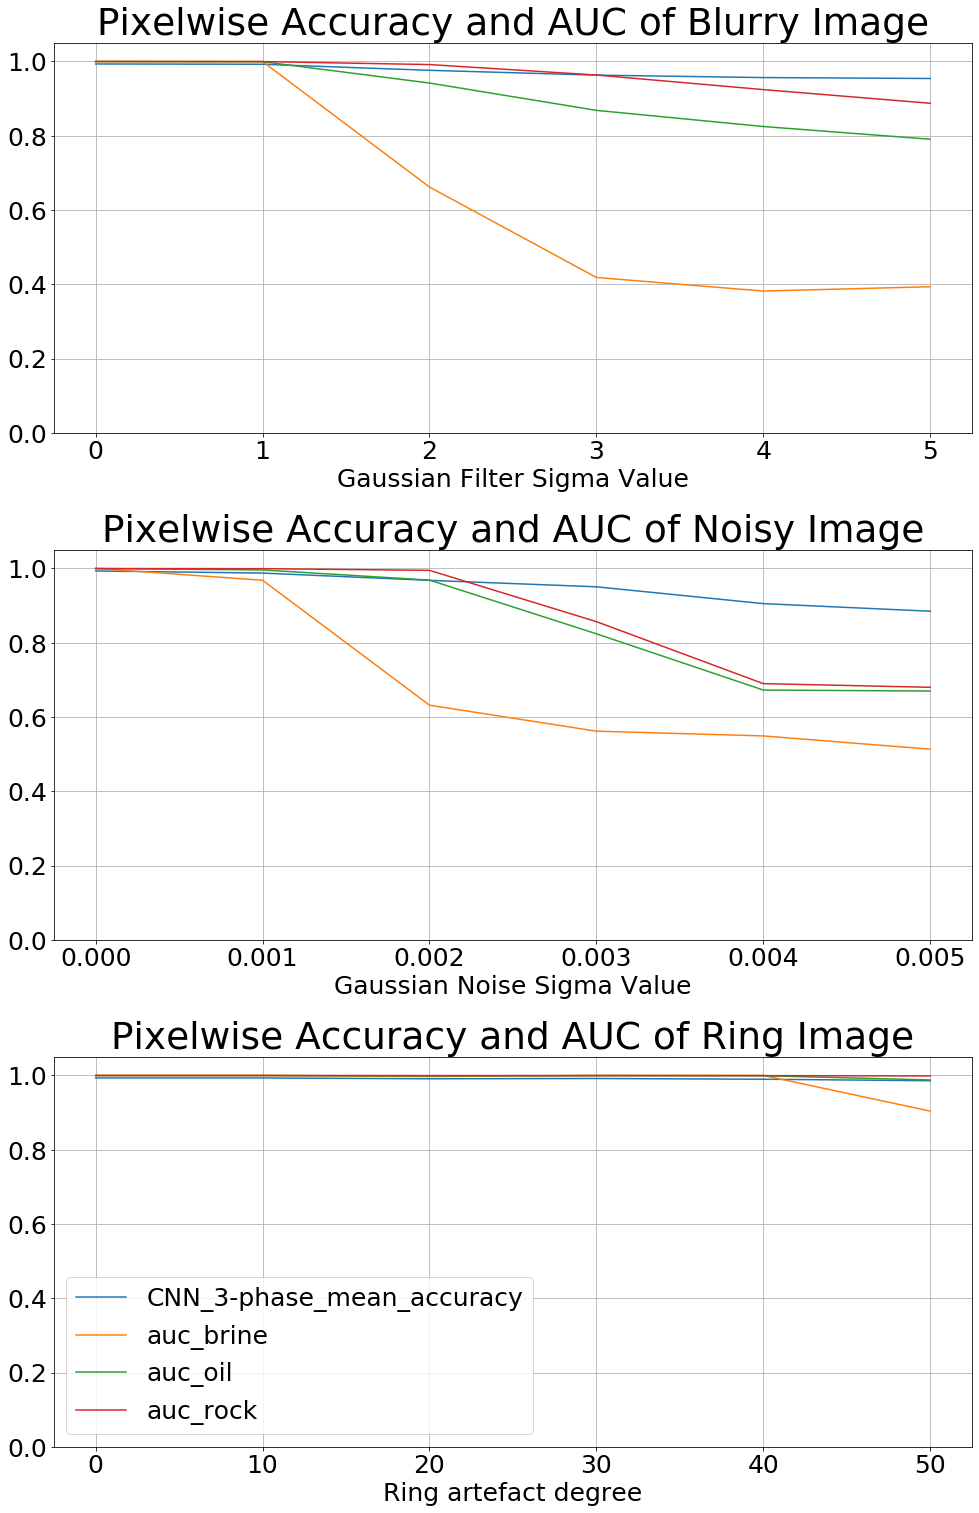
\includegraphics[width=33pc]{imgs/acc_auc.png}
 \caption{This figure shows the model's performance over three types of image degradation. For Gaussian filtered (blurred) images, the segmentation quality decreased a bit and stabilised. For Gaussian noised images, the segmentation quality plunged and no sign of stabilisation occured. For artificial ring artefacts, the segmentation quality is stable at a very high performance level, only minor decrease of performance at heavily degraded images.}
 \label{robustness}
 \end{figure}
 

\subsection{Future improvements}
Comparison of different network architectures can be further tested. Apart from the U-net, there are other powerful CNN architectures such as ResNet (\citet{he2016deep}), GoogLeNet (\citet{szegedy2015going}), VGGNet (\citet{simonyan2014very}) etc. with different advantages and specialities. It still remains to be tested on which is the most suitable architecture for segmenting \textmu \textmu CT images from multiphase fluid flow experiments.

The current training data set can be augmented by noising, mirroring, rotating, scaling, cropping or translating the original training images. Data augmentation allows amplification of the training data set based on currently existed data set and therefore further generalize the CNN model for more robust segmentation of different data sets. The data augmentation strategy was tested with the U-net architecture and produced excellent segmentation \citep{ronneberger2015u}. 

\subsection{Limitation}
As a prototype CNN network of segmenting \textmu CT data of core-flooding experiments, the current model learned mainly the segmentation process, rather than the intrinsic knowledge of 'what is rock' and 'what are fluids'. Because the training data itself is highly biased towards the particular rock and fluid type of this experiment. Different rocks have completely different internal structures. And the rock appearance on \textmu CT is highly dependent on the imaging settings, even the same rock can look different. Different fluids can vary in \textmu CT images too. The designed way of utility is to keep training on future experiments to generalise the model with more kinds of rocks and fluids. As more type of imaging conditions, noises, lithologies and fluid phases are collected in the training data, the model will be increasingly generalized as more varied data sets are provided. The future training needed will eventually decrease as the CNN network has 'seen' more rocks, fluids and experiments. That becomes the more mature model that can segment multiphase fluid flow experiment data regardless of noise, rock type, fluid type and beam line condition.

\section{Conclusion}
The CNN segmentation can significantly improve the segmentation workflow for multiphase flow \textmu CT images. The advantages are five-fold. Firstly once a network for segmenting multiphase flow images is trained, it can be applied to future data without re-train. Second, once a network is trained it can function without a high quality reference image at time zero, allowing segmentation of any data set that lacks such a reference. Thirdly the segmentation is the direct output from reconstruction image, and so the considerable time consumed by pre-processing (tuning of filtering, registration, masking etc.) is no longer required. This is significant because for fast synchrotron \textmu CT data set, the data processing time is considerably long compared with time used for interpretation. Fourthly, the algorithm is capable for highly noised images, which is extremely limiting for conventional processing paths. Finally, the performance of the CNN network improves as more data it has seen, it evolves itself when it is used. Overall the CNN segmentation is a powerful and efficient tool for \textmu CT image segmentation, especially for extra-large and noisy data set.

%Text here ===>>>

%%

%  Numbered lines in equations:
%  To add line numbers to lines in equations,
%  \begin{linenomath*}
%  \begin{equation}
%  \end{equation}
%  \end{linenomath*}



%% Enter Figures and Tables near as possible to where they are first mentioned:
%
% DO NOT USE \psfrag or \subfigure commands.
%
% Figure captions go below the figure.
% Table titles go above tables;  other caption information
%  should be placed in last line of the table, using
% \multicolumn2l{$^a$ This is a table note.}
%
%----------------
% EXAMPLE FIGURE
%
% \begin{figure}[h]
% \centering
% when using pdflatex, use pdf file:
% \includegraphics[width=20pc]{figsamp.pdf}
%
% when using dvips, use .eps file:
% \includegraphics[width=20pc]{figsamp.eps}
%
% \caption{Short caption}
% \label{figone}
%  \end{figure}
%
% ---------------
% EXAMPLE TABLE
%
% \begin{table}
% \caption{Time of the Transition Between Phase 1 and Phase 2$^{a}$}
% \centering
% \begin{tabular}{l c}
% \hline
%  Run  & Time (min)  \\
% \hline
%   $l1$  & 260   \\
%   $l2$  & 300   \\
%   $l3$  & 340   \\
%   $h1$  & 270   \\
%   $h2$  & 250   \\
%   $h3$  & 380   \\
%   $r1$  & 370   \\
%   $r2$  & 390   \\
% \hline
% \multicolumn{2}{l}{$^{a}$Footnote text here.}
% \end{tabular}
% \end{table}

%% SIDEWAYS FIGURE and TABLE
% AGU prefers the use of {sidewaystable} over {landscapetable} as it causes fewer problems.
%
% \begin{sidewaysfigure}
% \includegraphics[width=20pc]{figsamp}
% \caption{caption here}
% \label{newfig}
% \end{sidewaysfigure}
%
%  \begin{sidewaystable}
%  \caption{Caption here}
% \label{tab:signif_gap_clos}
%  \begin{tabular}{ccc}
% one&two&three\\
% four&five&six
%  \end{tabular}
%  \end{sidewaystable}

%% If using numbered lines, please surround equations with \begin{linenomath*}...\end{linenomath*}
%\begin{linenomath*}
%\begin{equation}
%y|{f} \sim g(m, \sigma),
%\end{equation}
%\end{linenomath*}

%%% End of body of article

%%%%%%%%%%%%%%%%%%%%%%%%%%%%%%%%
%% Optional Appendix goes here
%
% The \appendix command resets counters and redefines section heads
%
% After typing \appendix
%
%\section{Here Is Appendix Title}
% will show
% A: Here Is Appendix Title
%
%appendix
%\section{Jupyter Notebook}

%%%%%%%%%%%%%%%%%%%%%%%%%%%%%%%%%%%%%%%%%%%%%%%%%%%%%%%%%%%%%%%%
%
% Optional Glossary, Notation or Acronym section goes here:
%
%%%%%%%%%%%%%%
% Glossary is only allowed in Reviews of Geophysics
%  \begin{glossary}
%  \term{Term}
%   Term Definition here
%  \term{Term}
%   Term Definition here
%  \term{Term}
%   Term Definition here
%  \end{glossary}

%
%%%%%%%%%%%%%%
% Acronyms
%   \begin{acronyms}
%   \acro{Acronym}
%   Definition here
%   \acro{EMOS}
%   Ensemble model output statistics
%   \acro{ECMWF}
%   Centre for Medium-Range Weather Forecasts
%   \end{acronyms}

%
%%%%%%%%%%%%%%
% Notation
%   \begin{notation}
%   \notation{$a+b$} Notation Definition here
%   \notation{$e=mc^2$}
%   Equation in German-born physicist Albert Einstein's theory of special
%  relativity that showed that the increased relativistic mass ($m$) of a
%  body comes from the energy of motion of the body—that is, its kinetic
%  energy ($E$)—divided by the speed of light squared ($c^2$).
%   \end{notation}




%%%%%%%%%%%%%%%%%%%%%%%%%%%%%%%%%%%%%%%%%%%%%%%%%%%%%%%%%%%%%%%%
%
%  ACKNOWLEDGMENTS
%
% The acknowledgments must list:
%
% >>>>	A statement that indicates to the reader where the data
% 	supporting the conclusions can be obtained (for example, in the
% 	references, tables, supporting information, and other databases).
%
% 	All funding sources related to this work from all authors
%
% 	Any real or perceived financial conflicts of interests for any
%	author
%
% 	Other affiliations for any author that may be perceived as
% 	having a conflict of interest with respect to the results of this
% 	paper.
%
%
% It is also the appropriate place to thank colleagues and other contributors.
% AGU does not normally allow dedications.


\acknowledgments
 This study is funded by Petrobras and Royal Dutch Shell via International Centre for Carbonate Reservoirs. 


%% ------------------------------------------------------------------------ %%
%% References and Citations

%%%%%%%%%%%%%%%%%%%%%%%%%%%%%%%%%%%%%%%%%%%%%%%
% BibTeX is preferred:
%
\bibliography{aguref.bib}
%
% no need to specify bibliographystyle
%%%%%%%%%%%%%%%%%%%%%%%%%%%%%%%%%%%%%%%%%%%%%%%


% Please use ONLY \citet and \citep for reference citations.
% DO NOT use other cite commands (e.g., \cite, \citeyear, \nocite, \citealp, etc.).
%% Example \citet and \citep:
%  ...as shown by \citet{Boug10}, \citet{Buiz07}, \citet{Fra10},
%  \citet{Ghel00}, and \citet{Leit74}.

%  ...as shown by \citep{Boug10}, \citep{Buiz07}, \citep{Fra10},
%  \citep{Ghel00, Leit74}.

%  ...has been shown \citep [e.g.,][]{Boug10,Buiz07,Fra10}.


\end{document}



More Information and Advice:

%% ------------------------------------------------------------------------ %%
%
%  SECTION HEADS
%
%% ------------------------------------------------------------------------ %%

% Capitalize the first letter of each word (except for
% prepositions, conjunctions, and articles that are
% three or fewer letters).

% AGU follows standard outline style; therefore, there cannot be a section 1 without
% a section 2, or a section 2.3.1 without a section 2.3.2.
% Please make sure your section numbers are balanced.
% ---------------
% Level 1 head
%
% Use the \section{} command to identify level 1 heads;
% type the appropriate head wording between the curly
% brackets, as shown below.
%
%An example:
%\section{Level 1 Head: Introduction}
%
% ---------------
% Level 2 head
%
% Use the \subsection{} command to identify level 2 heads.
%An example:
%\subsection{Level 2 Head}
%
% ---------------
% Level 3 head
%
% Use the \subsubsection{} command to identify level 3 heads
%An example:
%\subsubsection{Level 3 Head}
%
%---------------
% Level 4 head
%
% Use the \subsubsubsection{} command to identify level 3 heads
% An example:
%\subsubsubsection{Level 4 Head} An example.
%
%% ------------------------------------------------------------------------ %%
%
%  IN-TEXT LISTS
%
%% ------------------------------------------------------------------------ %%
%
% Do not use bulleted lists; enumerated lists are okay.
% \begin{enumerate}
% \item
% \item
% \item
% \end{enumerate}
%
%% ------------------------------------------------------------------------ %%
%
%  EQUATIONS
%
%% ------------------------------------------------------------------------ %%

% Single-line equations are centered.
% Equation arrays will appear left-aligned.

Math coded inside display math mode \[ ...\]
 will not be numbered, e.g.,:
 \[ x^2=y^2 + z^2\]

 Math coded inside \begin{equation} and \end{equation} will
 be automatically numbered, e.g.,:
 \begin{equation}
 x^2=y^2 + z^2
 \end{equation}


% To create multiline equations, use the
% \begin{eqnarray} and \end{eqnarray} environment
% as demonstrated below.
\begin{eqnarray}
  x_{1} & = & (x - x_{0}) \cos \Theta \nonumber \\
        && + (y - y_{0}) \sin \Theta  \nonumber \\
  y_{1} & = & -(x - x_{0}) \sin \Theta \nonumber \\
        && + (y - y_{0}) \cos \Theta.
\end{eqnarray}

%If you don't want an equation number, use the star form:
%\begin{eqnarray*}...\end{eqnarray*}

% Break each line at a sign of operation
% (+, -, etc.) if possible, with the sign of operation
% on the new line.

% Indent second and subsequent lines to align with
% the first character following the equal sign on the
% first line.

% Use an \hspace{} command to insert horizontal space
% into your equation if necessary. Place an appropriate
% unit of measure between the curly braces, e.g.
% \hspace{1in}; you may have to experiment to achieve
% the correct amount of space.


%% ------------------------------------------------------------------------ %%
%
%  EQUATION NUMBERING: COUNTER
%
%% ------------------------------------------------------------------------ %%

% You may change equation numbering by resetting
% the equation counter or by explicitly numbering
% an equation.

% To explicitly number an equation, type \eqnum{}
% (with the desired number between the brackets)
% after the \begin{equation} or \begin{eqnarray}
% command.  The \eqnum{} command will affect only
% the equation it appears with; LaTeX will number
% any equations appearing later in the manuscript
% according to the equation counter.
%

% If you have a multiline equation that needs only
% one equation number, use a \nonumber command in
% front of the double backslashes (\\) as shown in
% the multiline equation above.

% If you are using line numbers, remember to surround
% equations with \begin{linenomath*}...\end{linenomath*}

%  To add line numbers to lines in equations:
%  \begin{linenomath*}
%  \begin{equation}
%  \end{equation}
%  \end{linenomath*}



